\subsection{Wiring an Ideal Space-Filling Hierarchical Tree with Log-Time Physical Interconnects} \label{sec:proof3}

Once more, we will work with a mesh of $n$ physical hardware nodes corresponding to a graph $N$ where $V(N)$ represents computational nodes and $E(N)$ represents physical interconnects between nodes.
In this case, in addition to physical interconnects between spatially adjacent nodes we will assume a system of hierarchical physical interconnects that allows log-hop traversal between nodes.

\begin{figure}[t]
\begin{center}
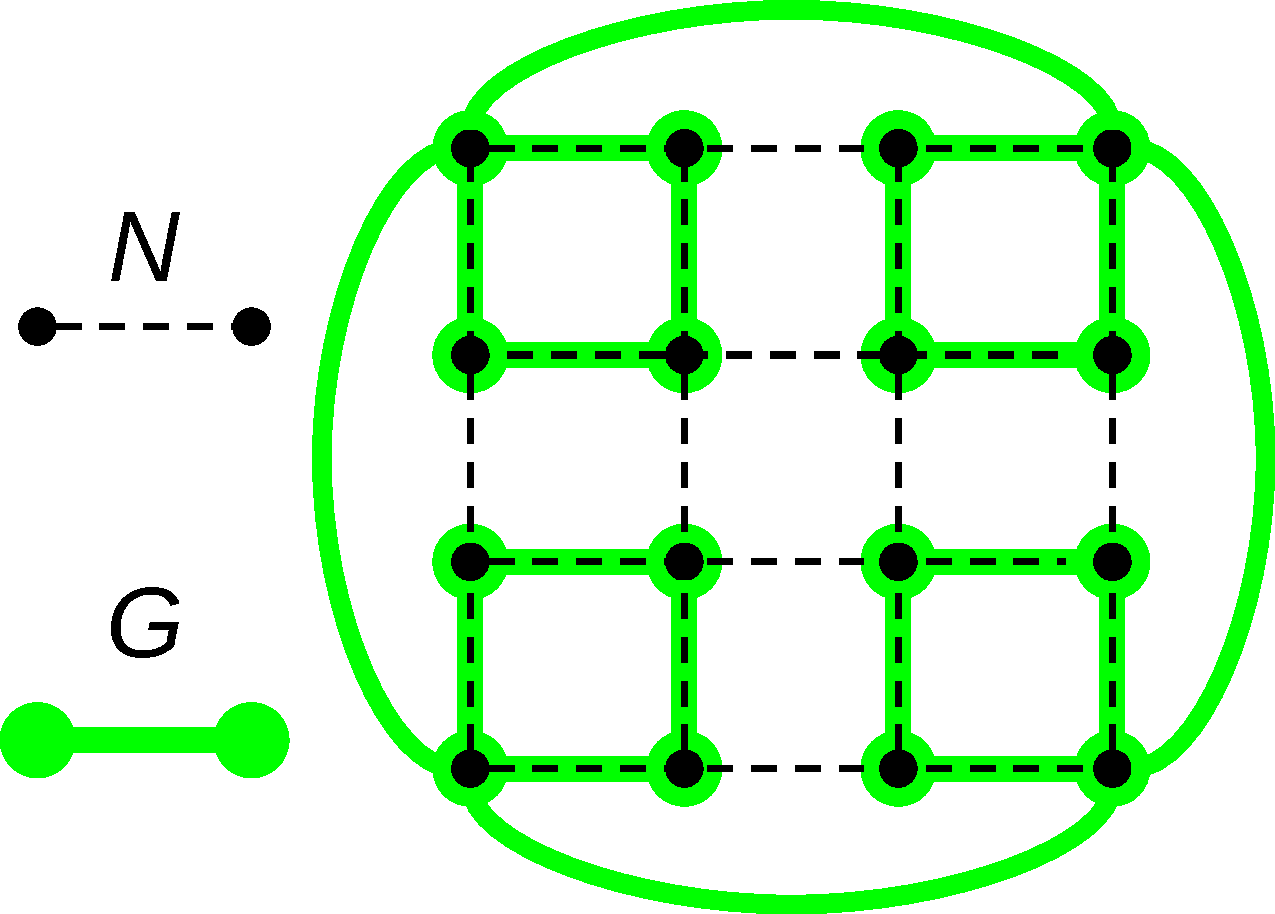
\includegraphics[width=\linewidth]{spacefilling}
\caption{
Example construction of an ideal space-filling tree over a computational mesh.
}
\label{fig:spacefilling}
\end{center}
\end{figure}


Suppose we have a small-world graph $G$ with maximum vertex degree bounded by a finite constant $m$.
The vertices of this graph $G$ are embedded one-to-one on $N$ such that $|V(G)| = |V(N)|$.
We will specifically construct this graph as an ideal space-filling tree.
Figure \ref{fig:spacefilling} illustrates the relationship between $N$ and $G$.

As a property of this construction, $|E(N)| \propto |V(N)|$.

In the best case, where edges in $E(G)$ happen to correspond exactly to hierarchical physical interconnects $E(N)$, the average hops required per edge is 1.
However, in the worst case the average number of hops over $N$ required per edge in $E(G)$ is bounded by $\log_m n$.

What if, instead of routing all traffic through log-time hierarchical interconnects, we routed traffic between nodes less than $\log_m n$ apart through local grid-mesh interconnects?

In this case, we can bound worst-case total wiring cost by
\begin{align*}
\sum_{l = 1}^{\log_2 \log_m n} % short edges
\Big[
  m^{\log_m n - l} % number of edges
  \times
  2^l % hop length
\Big]
+
\log_m n % number hops
\times
\sum_{l = \log_2 \log_m n }^{ \log_m n} % long edges
m^{\log_m n - l}.
\end{align*}

For the space-filling tree on a one-dimensional mesh, we have $m = 2$.
Our upper bound on total wiring cost simplifies to
\begin{align*}
w_2(n) =
n \times \log_2 \log_2 n
+
\log_2 n \times (n \times \log_n 4 - 1).
\end{align*}

Because
\begin{align*}
\lim_{n \rightarrow \infty}
\frac{
  w_2(n)
}{
  n \times \log_2 \log_2 n
}
= 1,
\end{align*}
we have $w_2(n) \in \Theta \Big( n \times \log_2 \log_2 n \Big)$.
Because edge count $|E(G)| \in \Theta \Big( n \Big)$ we can establish the following upper bound on $\bar{W}(n)$ mean wiring cost per edge in $|E(G)|$ for the one-dimensional case,
\begin{align*}
\bar{W}(n) \in \Omega\Big( \log_2 \log_2 n \Big).
\end{align*}

What about the three-dimensional case?
For the space-filling tree on a three-dimensional mesh, we have $m = 8$.
Our upper bound on total wiring cost simplifies to
\begin{align*}
w_8(n)
=&
\frac{n}{3}
\times (1 - 4^{ \log_2 \log_n 8 }) \\
&+
\frac{
  (
    n \times 8^{
      \log_2 \log_n 64
    } - 1
  ) \times \log_8 n
}{7}.
\end{align*}

Because
\begin{align*}
\lim_{n \rightarrow \infty}
\frac{
  w_8(n)
}{
  n
}
= \frac{1}{3},
\end{align*}
we have $w_8 \in \Theta \Big( n \Big)$.
Once more, because edge count $|E(G)| \in \Theta \Big( n \Big)$ we can establish the following upper bound on $\bar{W}(n)$ mean wiring cost per edge for the three-dimensional case,
\begin{align*}
\bar{W}(n) \in \Omega \Big( 1 \Big).
\end{align*}

% \begin{align*}
% \lim_{n \rightarrow \infty}
% \frac{\frac{ (n \times 8^{ \log_2 \log_n 64 } - 1) \times \log_8 n }{7}}{n} = 0
% \end{align*}
%
% \begin{align*}
% \lim_{n \rightarrow \infty}
% \frac{\frac{n}{3} \times (1 - 4^{ \log_2 \log_n 8 })}{n} = 1/3
% \end{align*}

Similar analysis concludes an equivalent result in the two-dimensional case.

% For $b = 4$ (two-dimensional case) this simplifies to,
% \begin{align*}
% n \times \Big( 1 - \log_n(4) \Big)
% +
% \frac{
%   (
%     n \times 4^{
%       \log_2 \log_n 16
%     } - 1
%   ) \times \log_4 n
% }{3}
% \end{align*}
%
% \begin{align*}
% \lim_{n \rightarrow \infty}
% \frac{   (     n \times 4^{       \log_2 \log_n 16     } - 1   ) \times \log_4 n }{n \times \Big( 1 - \log_n(4) \Big)} = 0
% \end{align*}
%
% \begin{align*}
% \lim_{n \rightarrow \infty} \frac{n \times \Big( 1 - \log_n(4) \Big)}{n} = 1
% \end{align*}
